\documentclass[../main.tex]{subfiles}
% !TEX root= ../main.tex

\begin{document}

% \subsection{What Programmers Want}

% \begin{itemize}
% 	\item \textbf{Low latency:} messages take very little time from sender to receiver.
% 	\item \textbf{High bandwidth:} we can send large amounts of data between processors and everyone can communicate at the same time.
% 	\item \textbf{Uniformity:} All processors and connections are equivalent.
% \end{itemize}

\subsection{Performance Consideration}

\begin{itemize}
	\item \textbf{Bisection bandwidth:} find the worst way to divide the processors into sets of \(\frac{P}{2}\) processors each \(\times\) the bandwidth.
\end{itemize}

\subsection{Network Topologies}

\subsection{Diameter, Bisection Bandwidth, and Port Number of Each Network}

\renewcommand{\arraystretch}{1.5}

\begin{center}
	\begin{tabular}{| c | c | c | c | c |}
		\hline
		\textbf{Network}       & \textbf{Diameter}                  & \textbf{Bisection bandwidth} & \textbf{\# ports} & \textbf{Latency}    \\
		\hline
		\hline
		\textbf{Ring Network}  & \(P/2\)                            & 2                            & 2                 & \(O(P)\)            \\
		\hline
		\textbf{Star Networks} & 1                                  & P                            & P                 & \(O(1)\)            \\
		\hline
		\textbf{ND Meshes}     & \(N \times (\sqrt[N]{P} - 1)\)     & \(\sqrt[N]{P^{N-1}}\)        & 2N                & \(O(\sqrt{P}),N=2\) \\
		\hline
		\textbf{ND Torus}      & \(\frac{N}{2} \times \sqrt[N]{P}\) & \(2\sqrt[N]{P^{N-1}}\)       & N/A               & \(O(\sqrt{P}),N=2\) \\
		\hline
		\textbf{ND Hypercubes} & \(\log_2{P} = N\)                  & \(\frac{P}{2}\)              & \(\log_2{P} = N\) & N/A                 \\
		\hline
	\end{tabular}
\end{center}

\subsubsection{Ring Network}

\begin{multicols}{2}
	\begin{itemize}
		\item \textbf{Advantages:} Simple
		\item \textbf{Disadvantages:}
		\begin{itemize}
		    \item Worst-case latency grows as \(O(P)\)
		    \item Easily congested --- limited bandwidth.
		\end{itemize} 
	\end{itemize}

	\begin{center}
		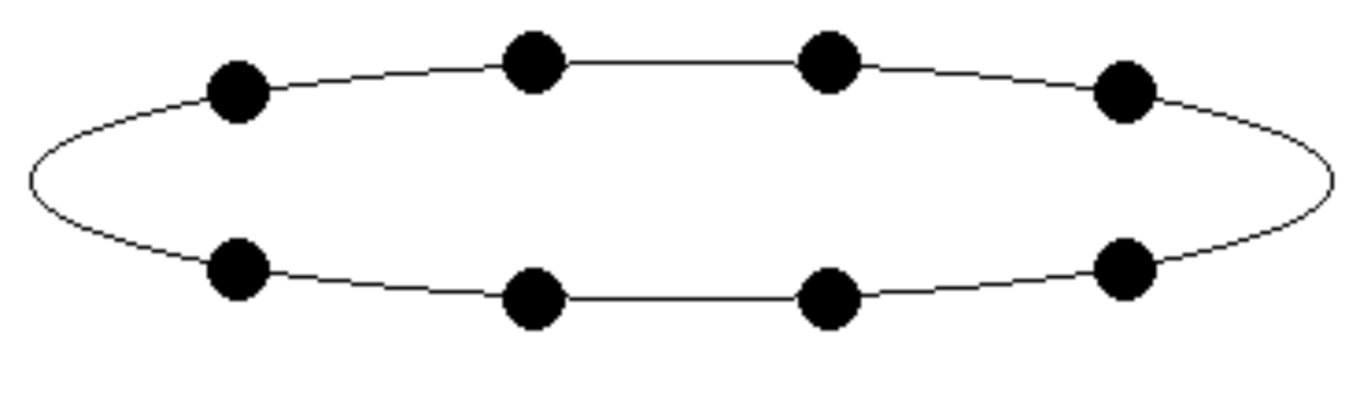
\includegraphics[scale=0.25]{ring-networks.png}
	\end{center}
\end{multicols}

\subsubsection{Star Networks}

\begin{multicols}{2}
	\begin{itemize}
		\item \textbf{Advantages:}
		      \begin{itemize}
			      \item \textbf{Low-latency:} single hop between any two nodes.
			      \item \textbf{High-bandwidth:} no contention for connections with different sources and destination
		      \end{itemize}
		\item \textbf{Disadvantages:}
		      \begin{itemize}
			      \item Amount of routing hardware grows as \(O(P^2)\).
			      \item Require lots of wires, to and from switch.
		      \end{itemize}
	\end{itemize}

	\begin{center}
		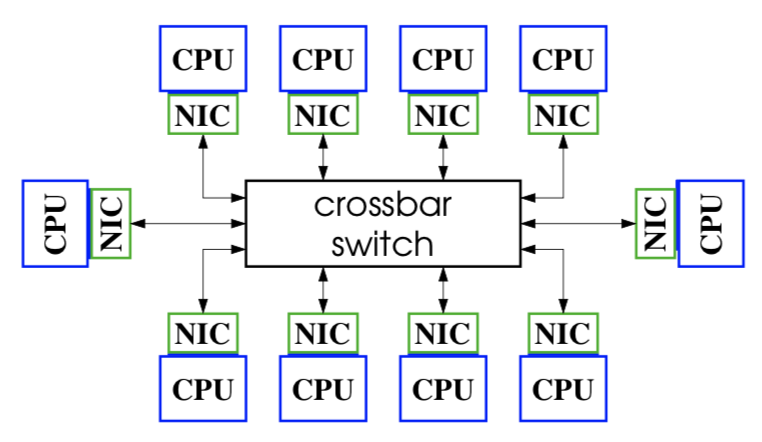
\includegraphics[scale=0.45]{star-networks.png}
	\end{center}
\end{multicols}

\subsubsection{Meshes}

\begin{multicols}{2}
	\begin{itemize}
		\item \textbf{Advantages:}
		      \begin{itemize}
			      \item \textbf{Easy to implement:} chips and circuits boards are effectively two-dimensional.
			      \item Cross-section bandwidth grow as \(\sqrt{P}\).
		      \end{itemize}
		\item \textbf{Disadvantages:}
		      \begin{itemize}
			      \item Worst-case latency grows as \(\sqrt{P}\).
			      \item Edges of mesh are "special cases".
		      \end{itemize}
	\end{itemize}

	\begin{center}
		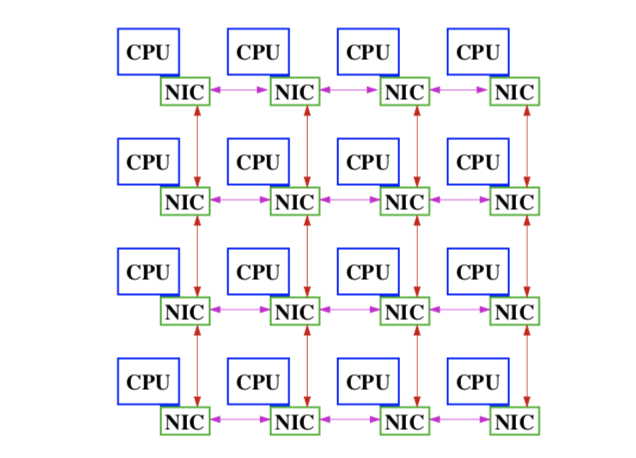
\includegraphics[scale=0.5]{2d-meshes.png}
	\end{center}
\end{multicols}


\subsubsection{Tori}

	\begin{center}
		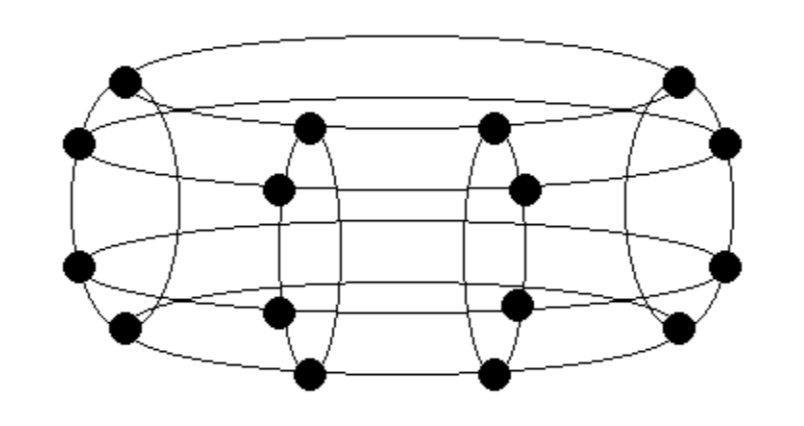
\includegraphics[scale=0.4]{2d-torus.png}
	\end{center}
\begin{multicols}{2}
	\begin{itemize}
		\item \textbf{Advantages:}
		      \begin{itemize}
			      \item Has the good features of a mesh.
			      \item No special cases at the edges.
			      \item Interconnect is simpler and takes less space.
			      \item more volume efficient
			      \item shorter wires save energy
			      \item make lower latency between neighbours
			      \item bounded degree nodes are more modular thus easier to implement
		      \end{itemize}
		      	\end{itemize}

		      	\begin{itemize}

		\item \textbf{Disadvantages:}
		      \begin{itemize}
			      \item Worst-case latency grows as \(\sqrt{P}\).
		      \end{itemize}
	\end{itemize}
\end{multicols}



\subsection{Hypercubes}

\begin{multicols}{2}
	\begin{itemize}
		\item \textbf{Advantages:}
		      \begin{itemize}
			      \item Small diameter \(\Rightarrow\) Small worst-case latency
			      \item high bisection bandwidth \(\Rightarrow\) fewer communication bottlenecks.
			      \item easily space shared
			      \item communication structure matches divide-and-conquer algorithms such bionic sort
			      \item more flexible routing avoids congestion
			      \item No special cases at edges.
		      \end{itemize}
		\item \textbf{Disadvantages:}
		      \begin{itemize}
			      \item Doesn't become "all wire“ for networks with a large number of processors.
		      \end{itemize}
	\end{itemize}

	\begin{center}
		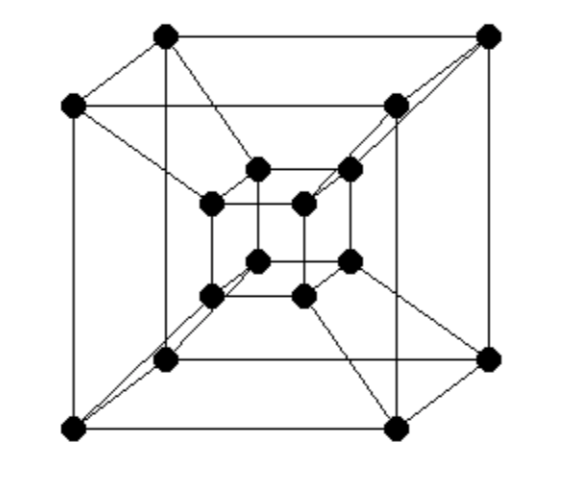
\includegraphics[scale=0.35]{hypercubes.png}
	\end{center}
\end{multicols}

\subsubsection{Trees}

\begin{center}
	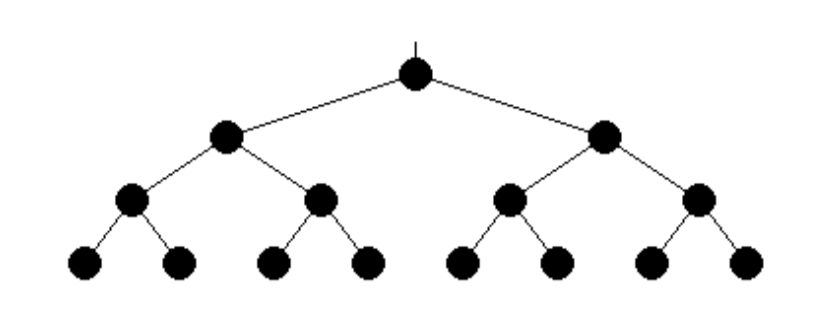
\includegraphics[scale=0.4]{binary-tree.png}
\end{center}

\begin{multicols}{2}

\begin{itemize}
	\item \textbf{Advantages:}
	      \begin{itemize}
		      \item Simple network: \# of routing nodes = \# of processors - 1
		      \item Wiring: \(O(\log_2{N})\) extra height, \(O(N\log_2{N})\) extra area.
		      \item \textbf{Low-latency:} \(O(\log_2{N}) +\) wire delay.
	      \end{itemize}
	\item \textbf{Disadvantages:}
	      \begin{itemize}
		      \item \textbf{Low-bandwidth:} bottleneck at root.
	      \end{itemize}
\end{itemize}

\begin{itemize}

	\item \textbf{Diameter and Bisection bandwidth}
	      \begin{itemize}
		      \item \textbf{Binary Tree}: P = 15, Diameter \(= 2\times \log_2{\frac{P+1}{2}} = 6\), Bisection bandwidth \(= 1\)
		      \item \textbf{3-ary Tree}: P = 13, Diameter \(= 4\), Bisection bandwidth \(= 3\)
		      \item \textbf{4-ary Tree}: P = 21, Diameter \(= 4\), Bisection bandwidth \(= 2\)
\end{itemize}

\end{itemize}

\end{multicols}

\subsubsection{Fat Trees}

% \begin{multicols}{2}

\begin{center}
	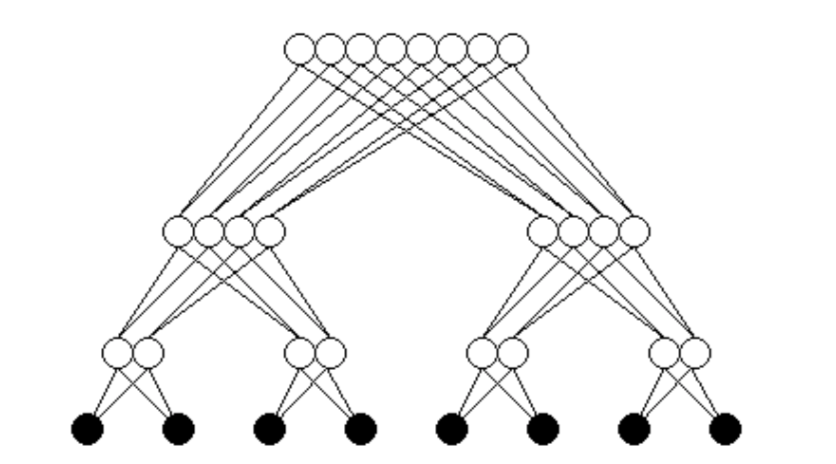
\includegraphics[scale=0.4]{fat-tree.png}
\end{center}

\begin{itemize}
	\item \textbf{Diameter and Bisection bandwidth}
	      \begin{itemize}
		      \item \textbf{Binary Fat Tree}: P = 8, Diameter \(= 2\times \log_2{P} = 6\), Bisection bandwidth \(= P\)
	      \end{itemize}
\end{itemize}

% \end{multicols}

\end{document}
